\documentclass[crop, multi = page]{standalone}
\usepackage[nomessages]{fp}
\usepackage{amsmath}
\usepackage{tikz}
\usetikzlibrary{calc}
\usetikzlibrary{decorations.pathreplacing}
\usetikzlibrary{patterns}

\usetikzlibrary{shapes.misc}

\usetikzlibrary{arrows.meta,arrows}
\usetikzlibrary{shapes.geometric}

\tikzset{cross/.style={cross out, draw=black, fill=none, minimum size=2*(#1-\pgflinewidth), inner sep=0pt, outer sep=0pt}, cross/.default={2pt}}

\begin{document}
\begin{page}
    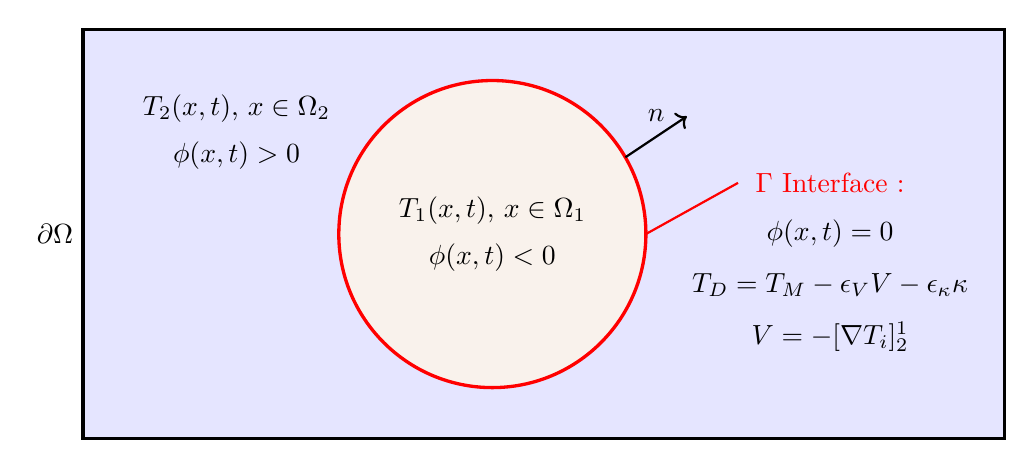
\begin{tikzpicture}[scale = 1.3]
    \draw[very thick, fill = blue!10] (0,0) rectangle (9,4);
    
    \draw[very thick, red, fill = brown!10] (4,2) circle (1.5);
    
    \draw (4,2) node[below] {$\phi(x, t) < 0$};
    \draw (4,2) node[above] {$T_1(x, t)$, $x \in \Omega_1$};
    \draw (1.5,3) node[below] {$\phi(x, t) > 0$};
    \draw (1.5,3) node[above] {$T_2(x, t)$, $x \in \Omega_2$};
    
    \draw (0,2) node[left] {$\partial \Omega$};
    
    \foreach \t [count=\k] in {{$V= -[\nabla T_i]^1_2$},
    {$T_D = T_M - \epsilon_V V - \epsilon_\kappa \kappa$},
    {$\phi(x, t) = 0$},
    {\color{red}$\Gamma$ Interface :}}
  {
   \node at ($(7.3,0.5 + \k/2)$){\t};
  }
    \draw[thick, ->] (5.3,2.75) to (5.9,3.15);
    
    \draw[thick, red, -] (5.5, 2) to (6.4, 2.5);
    
    \draw (5.6,3) node[above] {$n$};
    \end{tikzpicture}
 
\end{page}
\begin{page}
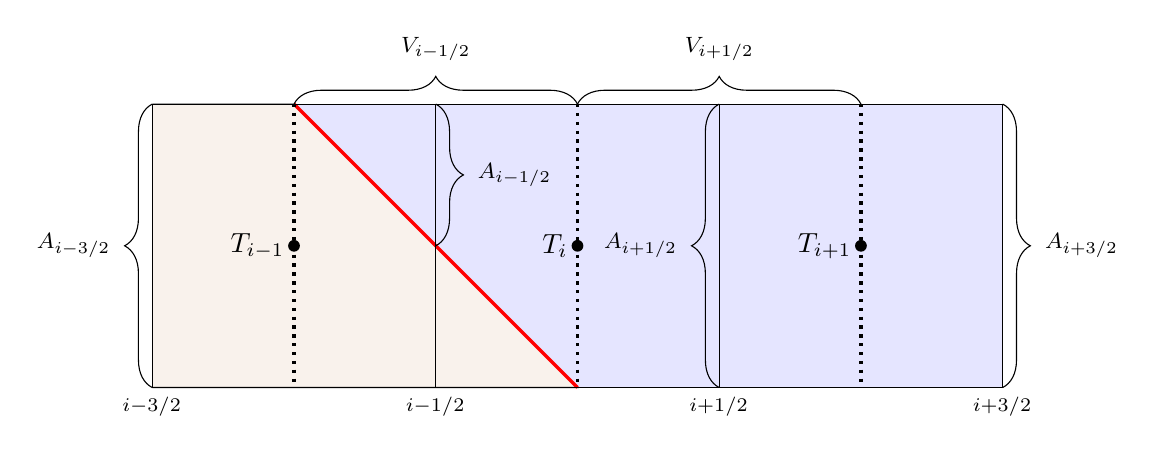
\begin{tikzpicture}[scale = 1.8]
    
    \draw[fill = blue!10] (-3,-1) rectangle (3,1);
    \draw[fill = brown!10] (-3,-1) -- (0,-1) -- (-2,1) -- (-3,1);
    
    \node at (-2,0) [circle,fill,inner sep=1.5pt]{};
    \node at (0,0) [circle,fill,inner sep=1.5pt]{};
    \node at (2,0) [circle,fill,inner sep=1.5pt]{};
    
    \draw (-2,0) node[left] {$T_{i-1}$};
    \draw (0,0) node[left] {$T_{i}$};
    \draw (2,0) node[left] {$T_{i+1}$};
    
    \draw [red, very thick] (-2,1) to (0,-1);
    \foreach \ii in {1,-1}
    	{\draw (-3,\ii) to (3,\ii);}
    \foreach \ii in {-3,1,-1,3}
    	{\draw (\ii,-1) to (\ii,1);}
    
    \draw [decorate,decoration={brace,amplitude=10pt,mirror}]
(-1,0) -- (-1,1) node [midway,xshift=1cm] {\footnotesize $A_{i-1/2}$};
	\draw [decorate,decoration={brace,amplitude=10pt}]
(1,-1) -- (1,1) node [midway,xshift=-1cm] {\footnotesize $A_{i+1/2}$};
\draw [decorate,decoration={brace,amplitude=10pt}]
(-3,-1) -- (-3,1) node [midway,xshift=-1cm] {\footnotesize $A_{i-3/2}$};

\draw [decorate,decoration={brace,mirror,amplitude=10pt}]
(3,-1) -- (3,1) node [midway,xshift=1cm] {\footnotesize $A_{i+3/2}$};

\draw [decorate,decoration={brace,amplitude=10pt}]
(-2,1) -- (0,1) node [midway,yshift=0.7cm] {\footnotesize $V_{i-1/2}$};

\draw [decorate,decoration={brace,amplitude=10pt}]
(0,1) -- (2,1) node [midway,yshift=0.7cm] {\footnotesize $V_{i+1/2}$};


\draw [dotted, very thick] (-2,1) to (-2,-1);
\draw [dotted, very thick] (0,1) to (0,-1);
\draw [dotted, very thick] (2,1) to (2,-1);


\draw (-3, -1) node[below] {$_{i-3/2}$};
\draw (-1, -1) node[below] {$_{i-1/2}$};
\draw (1, -1) node[below] {$_{i+1/2}$};
\draw (3, -1) node[below] {$_{i+3/2}$};

\end{tikzpicture}
\end{page}


\begin{page}
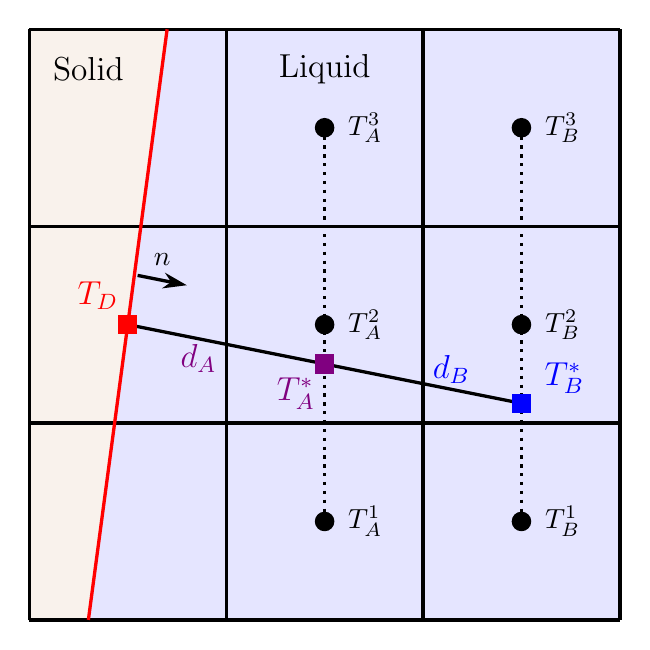
\begin{tikzpicture}[scale=2.5]
    
            \draw[fill = blue!10] (0,0) rectangle (3,3);
            \draw[fill = brown!10] (0.7, 3) -- (0.3, 0) -- (0,0) -- (0,3);
            
            \foreach \ii in {0, 1, 2, 3}
                	{\draw [very thick] (0, \ii) to (3,\ii);}
            \foreach \ii in {0, 1, 2, 3}
                	{\draw [very thick] (\ii, 0) to (\ii, 3);}
            
            \draw [very thick, red] (0.7, 3) to (0.3, 0);
            
            \foreach \ii in {0.5, 1.5, 2.5}
            	{\FPeval{\result}{clip(0.5 + \ii)}
            	\node at (1.5,\ii) [circle,fill,inner sep=2.5pt]{};
            	\node at (2.5,\ii) [circle,fill,inner sep=2.5pt]{};
            	\draw (1.5, \ii) node[right, xshift=5pt] {$T^{\result}_A$};
            	\draw (2.5, \ii) node[right, xshift=5pt] {$T^{\result}_B$};}
            	
            \draw [very thick, dotted] (2.5, 2.5) to (2.5, 0.5);
            \draw [very thick, dotted] (1.5, 2.5) to (1.5, 0.5);
            %1.5, 1.3
            %2.5, 1.1
            \draw [very thick] (0.5, 1.5) to (2.5, 1.1);
            
            \node at (0.5, 1.5) [red, rectangle,fill,inner sep=3.5pt]{};
            \node at (1.5, 1.3) [violet,fill,inner sep=3.5pt]{};
            \node at (2.5, 1.1) [blue,fill,inner sep=3.5pt]{};
            
            \draw [-{Stealth[length=3mm, width=2mm]}, very thick, black] (0.55, 1.75) to (0.8, 1.7);
            
            \draw (0.675, 1.725) node[above, yshift=2pt] {$n$};
            
            \draw (0.5, 1.5) node[red, left, yshift=10.5pt]{\large{$T_D$}};
            \draw (1.5, 1.3) node[violet, left, yshift=-10.7pt] {\large{$T^*_A$}};
            \draw (2.5, 1.1) node[blue, above, xshift=15.5pt] {\large{$T^*_B$}};
            
            \draw (2, 1.2) node[blue, right, yshift=5pt] {\large{$d_B$}};
            
            \draw (1, 1.4) node[violet,left, yshift=-5pt] {\large{$d_A$}};
            
            \draw (0.3, 2.8) node[] {\large{Solid}};
            \draw (1.5, 2.8) node[] {\large{Liquid}};
            
            \end{tikzpicture}
\end{page}

\begin{page}
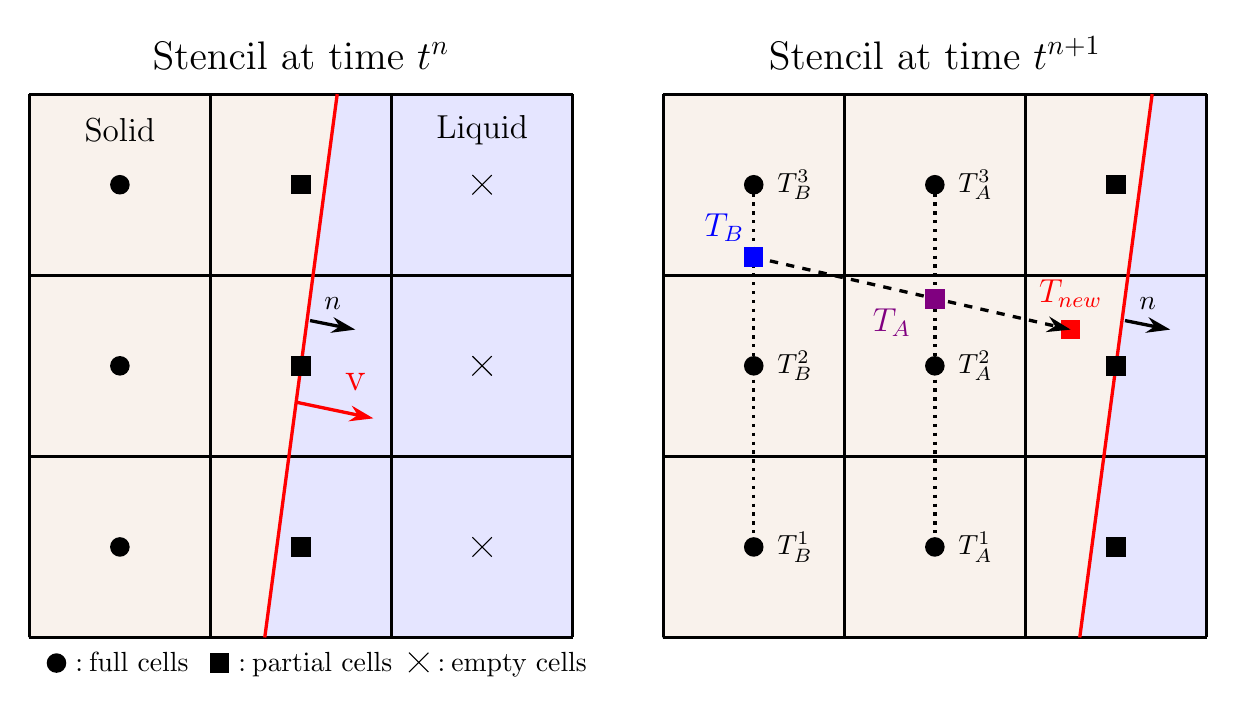
\begin{tikzpicture}[scale=2.3]

\draw[fill = blue!10] (0,0) rectangle (3,3);
\draw[fill = brown!10] (1.7, 3) -- (1.3, 0) -- (0,0) -- (0,3);

\foreach \ii in {0, 1, 2, 3}
    	{\draw [very thick] (0, \ii) to (3,\ii);}
\foreach \ii in {0, 1, 2, 3}
    	{\draw [very thick] (\ii, 0) to (\ii, 3);}

\draw [very thick, red] (1.7, 3) to (1.3, 0);


\foreach \ii in {0.5, 1.5, 2.5}
	{\node at (0.5,\ii) [circle,fill,inner sep=2.5pt]{};
	\node at (1.5,\ii) [rectangle,fill,inner sep=3.5pt]{};
	\node at (2.5,\ii) [cross, fill, inner sep=3.5pt]{};}


%1.5, 1.3
%2.5, 1.1
\draw [-{Stealth[length=3mm, width=2mm]}, very thick, red] (1.47, 1.3) to (1.9, 1.21);
\node at (1.8, 1.31) [above] {\Large{\textcolor{red}{v}}};

\draw (0.5, 2.8) node[] {\large{Solid}};
\draw (2.5, 2.8) node[] {\large{Liquid}};

\draw (1.5, 3) node[above, yshift=5.5pt] {\Large{Stencil at time $t^{n}$}};

\node at (0.15,0) [below, yshift=-5.5pt, circle, fill, inner sep=2.5pt]{}; 
\node at (0.2,0) [right, yshift=-8.75pt] {:$\:$full cells};

\node at (1.05,0) [below, yshift=-5.5pt, rectangle, fill, inner sep=3.5pt]{}; 
\node at (1.1,0) [right, yshift=-9.75pt] {:$\:$partial cells};

\node at (2.15,0) [below, yshift=-5.5pt, cross, fill, inner sep=3.5pt]{}; 
\node at (2.2,0) [right, yshift=-9.75pt] {:$\:$empty cells};

\draw [-{Stealth[length=3mm, width=2mm]}, very thick, black] (1.55, 1.75) to (1.8, 1.7);
            
\draw (1.675, 1.725) node[above, yshift=2pt] {$n$};
            
            
\begin{scope}[xshift = 3.5cm]
\draw[fill = blue!10] (0,0) rectangle (3,3);
\draw[fill = brown!10] (2.7, 3) -- (2.3, 0) -- (0,0) -- (0,3);

\foreach \ii in {0, 1, 2, 3}
    	{\draw [very thick] (0, \ii) to (3,\ii);}
\foreach \ii in {0, 1, 2, 3}
    	{\draw [very thick] (\ii, 0) to (\ii, 3);}

\draw [very thick, red] (2.7, 3) to (2.3, 0);


\foreach \ii in {0.5, 1.5, 2.5}
	{\node at (2.5,\ii) [rectangle, fill, inner sep=3.5pt]{};}

\foreach \ii in {0.5, 1.5, 2.5}
            	{\FPeval{\result}{clip(0.5 + \ii)}%
            	\node at (0.5,\ii) [circle,fill,inner sep=2.5pt]{};
            	\node at (1.5,\ii) [circle,fill,inner sep=2.5pt]{};
            	\draw (0.5, \ii) node[right, xshift=5pt] {$T^{\result}_B$};
            	\draw (1.5, \ii) node[right, xshift=5pt] {$T^{\result}_A$};}
%1.5, 1.3
%2.5, 1.1

\draw [very thick, dotted] (0.5, 2.5) to (0.5, 0.5);
\draw [very thick, dotted] (1.5, 2.5) to (1.5, 0.5);

\node at (2.25, 1.7) [rectangle,fill,inner sep=3.5pt, red]{};
\draw [-{Stealth[length=3mm, width=2mm]}, dashed, very thick,black]   (0.5, 2.1) to (2.25, 1.7);

\draw [-{Stealth[length=3mm, width=2mm]}, very thick, black] (2.55, 1.75) to (2.8, 1.7);

\draw (2.675, 1.725) node[above, yshift=2pt] {$n$};

%\draw [very thick] (2.25, 1.7)  to (0.5, 2.1);
\node at (0.5, 2.1) [rectangle,fill,inner sep=3.5pt, blue]{};
\node at (1.5, 1.87) [rectangle,fill,inner sep=3.5pt, violet]{};

\draw (2.25, 1.7) node[above, yshift=4.5pt, red] {\large{$T_{new}$}};
\draw (0.5, 2.1) node[left, yshift=10.5pt, blue] {\large{$T_B$}};
\draw (1.5, 1.87) node[below, xshift=-15.5pt, violet] {\large{$T_A$}};

\draw (1.5, 3) node[above, yshift=5.5pt] {\Large{Stencil at time $t^{n+1}$}};
\end{scope}


\end{tikzpicture}
\end{page}
\end{document}